\documentclass[twocolumn,oneside]{IEEEtran/IEEEtran}
% \documentclass[defaultstyle,11pt]{IEEETran}
% Lucy says to look at:
% float_page_fraction
% tex_page_fraction
% https://tex.stackexchange.com/questions/35125/how-to-use-the-placement-options-t-h-with-figures#35130
% \renewcommand\floatpagefraction{0.5} %% default: 0.5
% \renewcommand\topfraction{0.7} % default: 0.7
% \renewcommand*\textfraction{.05}
\usepackage{showframe}
\usepackage{amssymb}		% to get all AMS symbols
\usepackage{amsthm}
\usepackage{mathtools}
\usepackage{graphicx}		% to insert figures
% \usepackage{hyperref}		% PDF hyperreferences??
\usepackage{multirow}
\usepackage{mathtools}
\usepackage{cite}
\usepackage{listings}
\usepackage{booktabs}
% \usepackage{amsthm}
\usepackage[percent]{overpic}
\usepackage{caption}
\usepackage{subcaption}
\usepackage{xspace}
\usepackage{enumitem}
\usepackage{catchfilebetweentags} % for data input
\usepackage[inkscapelatex=false, inkscapepath=svgsubpath]{svg}
\usepackage{url}
\usepackage{mdframed}
\usepackage{amsmath, dsfont, bbold}
% \usepackage{algpseudocode,algorithm,algorithmicx}
\usepackage[ruled,linesnumbered]{algorithm2e}
\usepackage{placeins}
\usepackage{todonotes}

% Indent paragraphs inside enumerate
\usepackage{enumitem}
\setlist{  
  listparindent=\parindent,
  parsep=0pt,
}
\newcommand{\xyc}{\ensuremath{XY}\xspace}
\newcommand{\xc}{\ensuremath{X}\xspace}
\newcommand{\yc}{\ensuremath{Y}\xspace}
\newcommand{\zc}{\ensuremath{Z}\xspace}

\newcommand{\rzup}{\ensuremath{r_{z,\textrm{up}}}\xspace}
\newcommand{\rzs}{\ensuremath{r_{z,\textrm{s}}}\xspace}


% *******************************************************************************
% This artificially increases the papersize and margins, so todo notes are legible.
% ***************** WARNING: comment this out for final version. ****************
\usepackage[paperwidth=734.295pt, textwidth=516pt,
            marginparsep=5pt, hoffset=10pt, marginparwidth=90pt,
            textheight=696pt]{geometry}
% Use layouts to display the original dimensions, so we can get as close to that as possible with
% our fake page size.
\usepackage{layouts}
%textwidth: \printinunitsof{in}\prntlen{\textwidth}
%linewidth: \printinunitsof{in}\prntlen{\linewidth}
% textwidth: \printinunitsof{in}\prntlen{\textheight}

% *******************************************************************************



%%%%%%%%%%%%%%%%%%%%%%%%%%%%%%%%%%%%%%%%%%%%%%%%%%%%%%%%%%%%%%%%%
%%%%%%%%%%%%%%%       BEGIN DOCUMENT...         %%%%%%%%%%%%%%%%%
%%%%%%%%%%%%%%%%%%%%%%%%%%%%%%%%%%%%%%%%%%%%%%%%%%%%%%%%%%%%%%%%%

\begin{document}
\title{Improving the Image Acquisition Rate of an Atomic Force Microscope Through Compressive Sampling}

\author{Roger A. Braker, Yufan Luo, Lucy Y. Pao and Sean B. Andersson
  \thanks{The authors are with the Dept. of Electrical, Computer, and Energy
    Engineering at the University of Colorado, 425 UCB, Boulder, CO 80309,
    United States. Phone: +1 (303) 492-2360. Fax: +1 (303) 492-2758. R. A.
    Braker (corresponding author roger.braker@colorado.edu) is a graduate
    student and L.Y. Pao (pao@colorado.edu) is the Richard \& Joy Dorf
    Professor.} \thanks{This work was supported in part by the US National
    Science Foundation (NSF Grant CMMI-1234980) and Agilent Technologies, Inc.}
}

\maketitle
\begin{abstract}
  Undersampling-based approaches in Atomic Force Microscopy (AFM) aim to reduce
  the time to acquire an image by reducing the number of measurements needed
  while still maintaining image quality. In this paper, we describe a hardware
  implementation and demonstration of one such approach based on the use of
  collections of short scans known as $\mu$--paths. Using a commercial AFM, we
  acquire data on a grating sample.
  %using two different sampling
  %approaches: randomly-placed $\mu-$paths and $\mu-$paths designed to minimize
  %the reconstruction error based on partial prior information about the spatial
  %frequency content in the sample image.
  Reconstructions are made from these data using
  %three approaches: (1) inpainting, an interpolation technique that
  %diffuses information from sampled locations into unsampled regions, (2)
  %basis-pursuit, a compressive sensing-based algorithm that seeks to minimize a
  %measure of sparsity in the underlying image, and (3)
  a new variant of basis
  pursuit, Basis Pursuit with Vertical Variation (BPVV), that is designed to reduce
  artifacts arising from the sampling pattern. The quality of the resulting
  images is compared to images from standard raster scans of the same regions at
  comparable imaging rates using both the peak signal-to-noise ratio and the
  structured similarity index metric
  and a new metric we call the relative damage index.
  \todo{Will this conclusion still hold?}
  These experiments demonstrate that at slow
  scan rates, the $\mu-$path scheme produces similar image quality with
  significantly less sampling (and thus less tip-sample interaction) and that at
  high rates, the undersampling scheme produces higher quality images than
  raster scanning.
\end{abstract}

\section{Introduction}\label{sec:introduction}
% textwidth: \printinunitsof{pt}\prntlen{\textwidth}

% linewidth: \printinunitsof{pt}\prntlen{\linewidth}

% paperwidth: \printinunitsof{pt}\prntlen{\paperwidth}

% marginparwidth: \printinunitsof{pt}\prntlen{\marginparwidth}

% marginsep: \printinunitsof{pt}\prntlen{\marginparsep}

% textheight: \printinunitsof{pt}\prntlen{\textheight}

The Atomic Force Microscope (AFM) is a powerful instrument capable of imaging
sample surface topography, material characteristics, and other surface
properties, at the nanometer scale. AFMs acquire information about the sample
through a variety of imaging modes, all of which rely on the deflection of the
cantilever caused by the tip-sample interaction force. While the details of each
of the modes are quite different, in general, feedback control is used to hold
the deflection signal constant and information about the property of interest is
inferred from the applied control or the measured dynamics of the cantilever
\cite{Abramovitch:2007gt}. Because of its versatility, spatial resolution, and
ability to image in vacuum, air, and liquid, AFM is widely used in a variety of
disciplines, including physics, biology and materials science
\cite{Dufrene:2017gm,Yang:2017im,Payton:2016hj,Altman:2015ic,Haase:2015eh}
	
In addition to imaging static samples, AFM is increasingly being applied to
study dynamics in systems with nanometer-scale features
\cite{Yang:2017im,Shibata:2017da,Shibata:2015jd,Ando:2014ja}. The image
acquisition time of conventional AFMs, however, is typically on the order of
seconds to minutes, severely limiting the time-scales that can be explored.
Driven by the need for faster imaging, there continue to be many active research
efforts to overcome this challenge. Since an AFM is fundamentally a mechanical
microscope, many of the approaches to high-speed AFM (HS-AFM) have focused on
modifications to the physical components. These have included the use of small,
fast cantilevers \cite{viani1999fast, braunsmann2010high,Adams:2016hg}, the
development of faster actuators \cite{Maroufi:2015gt,Yong:2012kd,Kenton:2012cm},
as well as the application of advanced controllers
\cite{Rana:2018es,Yong:2015gr,butterworth2010adaptive,salapaka2002high}. By
combining different techniques, there are current generation, high-end
instruments that can image at rates on the order of 1-10 frames/sec
\cite{Ando:2014ja}. However, the fastest rates are achieved only over small scan
ranges and there remain many systems of interest whose dynamics are faster even
than these instruments can achieve. In addition, there is a large installed base
of much slower AFMs that can benefit from alternative approaches to improving
imaging rate.
	
A complimentary class of HS-AFM approaches considers modifications to the
sampling scheme rather than the system mechanics. Alternative scan trajectories
like spirals, cycloids, and Lissajous figures, have been used in place of the
standard raster scan. These trajectories are easier for the actuators to follow,
allowing the tip to be moved more quickly and leading to faster image
acquisition on an otherwise unmodified instrument
\cite{Bazaei:2017dm,Wu:2015dt,Rana:2014bj,Tuma:2012hv,Yong:2010gm}. Such
approaches are ultimately limited by the vertical bandwidth of the instrument
for regulating the deflection signal \cite{Teo:2016ev}. Related to these are
local scanning methods that use the measurements in real-time to steer the tip
to focus the scan on features of interest, reducing imaging time by reducing the
amount of sampling needed
\cite{Hartman:2018ja,Wen:2018fl,Zhang:2015cf,Huang:2014dw}. While these have
been shown to yield an order of magnitude or better improvement in imaging rate,
they are limited in the class of samples that can be imaged.
	
An alternative group of non-raster scanning schemes, introduced in
\cite{song2011video,andersson2012non}, is based on the idea of undersampling. As
with local scanning, data acquisition time is reduced by reducing the amount of
measurements acquired. Unlike local scanning methods, this approach still
presents the full image. Taking advantage of the redundancy in many natural
signals of interest, the final surface image can be recovered from the limited
number of measured pixels using a variety of different reconstruction methods
such as inpainting or schemes based on the theory of compressive sensing (CS)
\cite{chen2013enhancement,luo2015comparison}. In addition to the reduced imaging
time, undersampling schemes also reduce tip-sample interactions, thereby
reducing the likelihood of tip wear or sample damage.
	
One simple way to create undersampling schemes is by modifying existing full
scan patterns including raster, spiral, and Lissajous scanning. For example,
subline sampling is generated by randomly skipping some of the horizontal lines
in raster scanning \cite{han2018reconstruction,chen2013enhancement}. For spiral
and Lissajous patterns, the scan parameters (frequency and amplitude) can be
selected to ensure the trajectory only passes through a desired fraction of the
pixels in the final image. The scanning time for these smooth undersampling
patterns can be estimated based on the proportion of the pixels in the
trajectory. However, results in the literature of CS make clear that
\textit{randomness} in the sampling pattern is essential for creating good
reconstructions in the general case. The smooth nature of these patterns reduces
their randomness and thus leads to less accurate reconstructions than a
completely random sampling of the pixels for the same sampling fraction.
	
In AFM, implementing a truly random pattern requires that the tip be engaged
with the surface to collect a measurement, lifted and moved to the new location,
and engaged again. Because the re-engagement process is typically slow, this can
lead to excessively long image acquisition times and negate the gains from
undersampling \cite{andersson2012non}. One discrete undersampling scheme, called
a $\mu$-path pattern, was proposed in \cite{maxwell2014compressed} to improve
sampling efficiency. The $\mu$-path pattern consists of randomly placed short,
horizontal scans (see Fig.~\ref{fig:mu_mask} for one such pattern) and is
designed to balance the randomness needed to ensure good reconstruction with
continuous scanning to reduce the number of tip
engagements. %Though the pattern is motivated from CS, it also works well in practice for inpainting reconstruction \cite{luo2015comparison}.
\todo{Would be beneficial to shrink intro, if possible}

Our previous work on the $\mu$-path pattern using theoretical calculations,
simulations, and a preliminary implementation, demonstrates that the approach
can achieve significant scanning time reduction while maintaining faithful image
reconstruction \cite{maxwell2014compressed,Luo:2015tu, braker_hardware_2018}. This paper
builds upon that earlier work in several significant ways.
% % ------------------ TKTKTKT ------------------
% \todo{Strike this?}
% First, we demonstrate
% performance using both randomly-placed $\mu-$paths and designed $\mu-$paths that
% are optimized to minimize the expected reconstruction error given some initial
% estimate of the frequency structure of the sample. These schemes are described
% in Sec. \ref{sec:samplingScheme}.
% % --------------------------
We also introduce a new reconstruction
algorithm which is designed to minimize the artifacts arising from the structure
of the $\mu$-path scanning pattern. This algorithm is described and compared to
existing reconstruction methods through simulations in Sec.
\ref{sec:reconstructionMethods}.
Section \ref{sec:control} describes improvements to the control algorithms compared to our preliminary implementation in ~\cite{braker_hardware_2018}.
We then demonstrate the entire scheme from
sampling through reconstruction using experiments on a commercial AFM (Agilent
5500). The experimental setup and implementation details are described in Secs.
\ref{sec:experimentalSetup} and \ref{sec:implementation}\footnote{The software
  portion of the implementation and image reconstruction described in this paper
  can be found at \url{https://github.com/rabraker/AFM_CS}}. Experimental results are provided in Sec.
\ref{sec:results}. Finally, we provide a few concluding remarks in
Sec. \ref{sec:conclusions}.

\begin{figure}
  \centering
  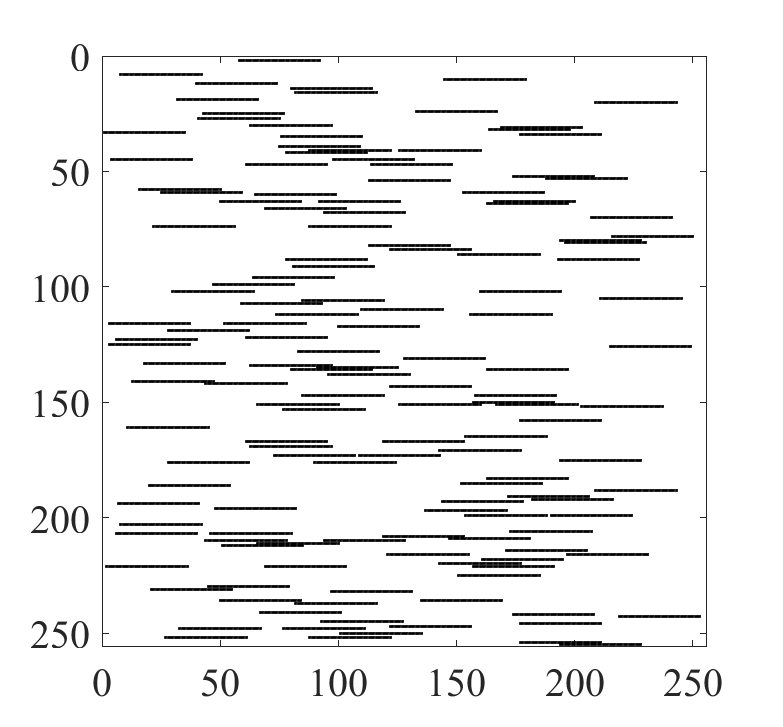
\includegraphics[width=0.7\columnwidth]{figures-SBA/random_mask.pdf}
  \caption{An example of the horizontal $\mu$-path sampling pattern for a 256$\times$256 pixel image with 35 pixels in each short scan and a total of 20\% pixels scanned.}
  \label{fig:mu_mask}
\end{figure}
% =========================================================================
\subsection{Reconstruction methods}
\label{sec:reconstructionMethods}
Compressive sensing (CS) is a signal processing technique which aims at signal reconstruction from a
relatively small (sub-Nyquist limit) number of measurements
\cite{carmi2014compressive}. It takes advantage of the approximate sparsity of
real-world signals, that is, that many coefficients of such signals
are close to zero when represented in an appropriate basis. CS methods seek the
true image signal $x\in\mathbb{R}^n$ from the observation equation,
\begin{equation}\label{op:observation}
  y = R x = RU\eta,
\end{equation}
\noindent where $y\in\mathbb{R}^n$ is the observation vector, $R$ is an
$n\times m$ matrix defining the measurements, $U$ is an $m\times m$ sparsity
basis and $\eta$ is the sparse representation of $x$ in the domain of $U$. In
general, $n\ll m$. In an imaging application, where the underlying signal is a
matrix $X\in\mathbb{R}^{h\times s}$, we take $x=\text{vec}(X)$, where the
$\text{vec}(\cdot)$ operator stacks the columns of a matrix.

	
In the AFM application, the probe can only measure a single pixel at a time.
Thus the rows of $R$ are a subset of the rows of an $m$ by $m$ identity matrix.
Ideally, the sparsity basis and
the measurement matrix $R$ will have a low \textit{mutual coherence}, a
measure that describes how each of the rows of $R$ (the measurements)
``spreads out'' in the domain of $U$ \cite{candes2007sparsity}.
In the following, we assume that $U^TU=I$, though in the simulation and
experimental results, we take $U$ as the Discrete Cosine Transform (DCT) basis.
The DCT basis generally keeps a good balance between achieving a low
mutual coherence between $U$ and the required structure of the AFM sensing
matrices $R$ and providing a high sparsity of typical AFM sample images. 
	
Basis pursuit with denoising (BPDN) is one common realization of the CS-based
reconstruction problem, and is given by the optimization
\begin{equation}
  \min_{x} \left \| U^Tx \right \|_1 \quad
  \text{s.t.}\quad x\in Q_p = \{x:~\|Rx - y\|_2 < \sigma\} \label{op:bp}
\end{equation}
where $\sigma$ represents uncertainty in the measurements. BPDN
essentially searches for the sparsest signal from all
the candidates that match the measurements.

Although BPDN is effective in the general setting, using it for reconstruction
from horizontal $\mu$-path samples often yields artifacts in the vertical
direction (that is, the direction orthogonal to the $\mu$-path scans) leading to
strong discontinuities in the image. These artifacts grow more prominent as the
length of the $\mu$-paths is increased \cite{maxwell2014compressed} as these
longer paths lead to increased mutual coherence between the measurement matrix
$R$ and the sparsity basis $U$. However, longer $\mu$-paths means fewer
tip re-engagements and thus shorter scan times.
\noindent 
\begingroup \setlength{\tabcolsep}{1pt}
\begin{figure*}[h!]
  \centering
  \begin{tabular}{cccccc}
    \textit{\small original image} & \textit{\small BPDN} & \textit{\small BPVV}
    & \textit{\small detail of original} & \textit{\small detail of BPDN} & \textit{\small detail of BPVV} \\
    % 
    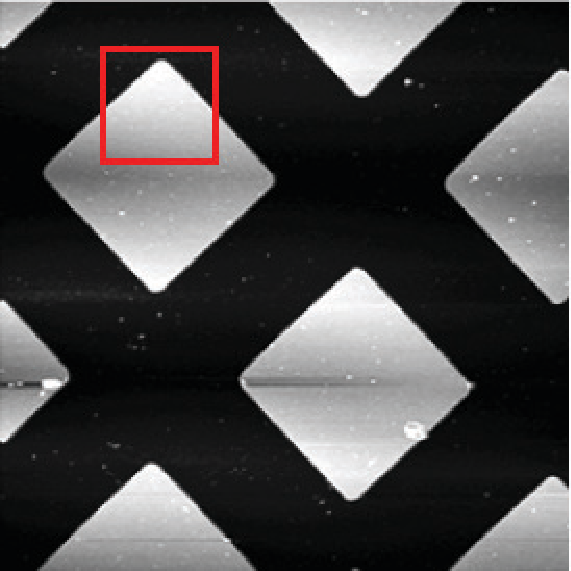
\includegraphics[width=0.16\textwidth]{figures-SBA/anothergrating_gt_framed}
    %
    & 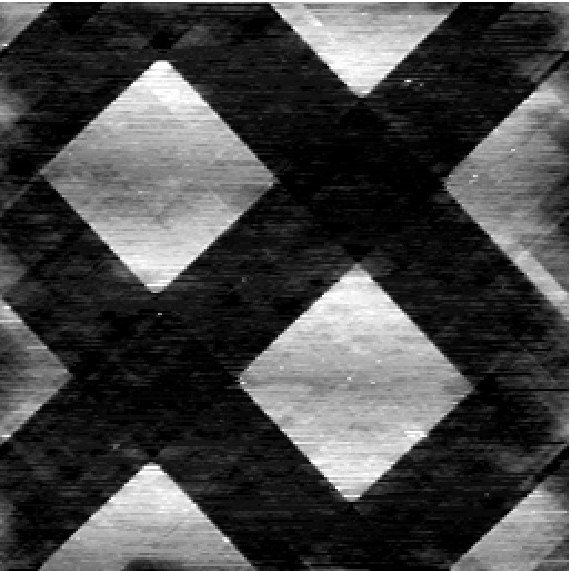
\includegraphics[width=0.16\textwidth]{figures-SBA/anothergrating_40mu}
     % 
    & 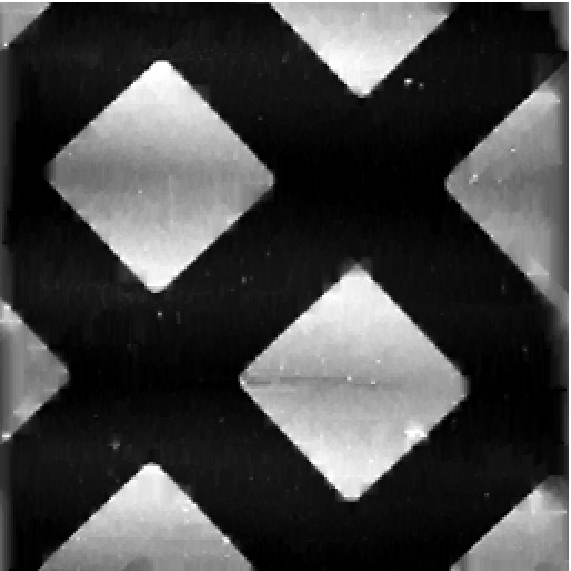
\includegraphics[width=0.16\textwidth]{figures-SBA/anothergrating_bptv_40mu}
     % 
    & 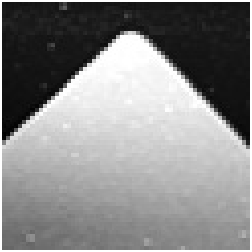
\includegraphics[width=0.16\textwidth]{figures-SBA/anothergrating_gt_zoomin}
     % 
    &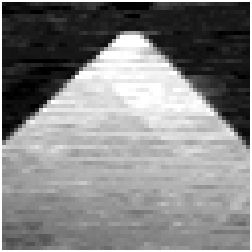
\includegraphics[width=0.16\textwidth]{figures-SBA/anothergrating_40mu_zoomin}
    %
    &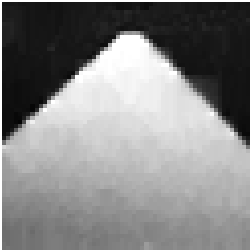
\includegraphics[width=0.16\textwidth]{figures-SBA/anothergrating_bptv_40mu_zoomin}\\
    % 
    % ------------------------------ Row  2 --------------------------------------------
    \includesvg[width=0.16\textwidth]{figures/dna_og.svg}
    %
    & \includesvg[width=0.16\textwidth]{figures/dna_bp.svg}
    %
    & \includesvg[width=0.16\textwidth]{figures/dna_bptv.svg}
    %
    & \includesvg[width=0.16\textwidth]{figures/dna_og_zoom.svg}
    %
    & \includesvg[width=0.16\textwidth]{figures/dna_bp_zoom.svg}
    %
    & \includesvg[width=0.16\textwidth]{figures/dna_bptv_zoom.svg}
  \end{tabular}
  \caption{Reconstruction comparison between BPDN and BPVV. (first column)
    Original raster-scanned image. (second column) BPDN reconstruction from
    random, 40 pixel long $\mu$-paths with 25\% sampling. (third column) BPVV
    reconstruction from the same sub-sampled data. (remaining columns)
    Corresponding details from the red boxes indicated in the raster image. The
    results show that BPVV reduces the artifacts arising from the horizontal
    scans of the $\mu$-path pattern that appear in BPDN reconstructions.}
  \label{fig:BPTV_demonstration}
\end{figure*}
\todo{Re-do this figure???}
\endgroup

\todo{This development is way too long!}
To mitigate these affects, we propose a new variant of BPDN that we term basis pursuit with
vertical variation (BPVV). BPVV adds a vertical total variation penalty in the spatial domain to the
optimization objective. That is, \eqref{op:bp} is modified to
\todo{It has been my observation that some benefit is gained by including $D_h$, but weighting it less than $D_v$. Not sure if we should leave it in. If so, BPVV should be BPTV or something.}
\begin{align}
  \min_{x\in Q_p}~f(x) &= \min_{x\in Q_p} \left\|U^Tx\right\|_1
                         + \alpha\left\|D_vx\right\|_1
                         + \beta\left\|D_hx\right\|_1 \label{op:bp_tv}\\
                       &=\min_{x\in Q_p} \left\|Wx\right\|_1 \label{op:bp_tvW}
                         % \quad W = \begin{bmatrix}U&\alpha_hD^T_h&\alpha_vD^T_v \end{bmatrix}^T \nonumber
\end{align}
where
\begin{equation*}
W = \begin{bmatrix}U&\alpha_hD^T_h&\alpha_vD^T_v \end{bmatrix}^T
\end{equation*}
with ${D_v x=\text{vec}(\nabla_v X)}$ (resp., ${D_v x=\text{vec}(\nabla_v X)}$) representing a 
discrete gradient of a matrix in the vertical (resp., horizontal) direction (see, e.g., \cite[Section 6.1,]{becker_nesta_2011}). 
% and
% \begin{align*}
%   (\nabla_v X)_{i,j} = 
%   \begin{cases}
%     X_{i+1,j} - X_{i,j}, & 1\leq i<h,~ 1\leq j\leq s,\\
%     0, & \phantom{:}i=h,~\phantom{:::::} 1\leq j\leq s.
%   \end{cases}\\
%   (\nabla_h X)_{i,j} = 
%   \begin{cases}
%     X_{i,j+1} - X_{i,j}, & 1\leq i\leq h,~1\leq j<s \\
%     0, & \phantom{}1\leq i\leq,~\phantom{:::} j=s
%   \end{cases}
% \end{align*}
Thus, in \eqref{op:bp_tv}, $\left \| D_v x \right \|_1$ (resp., $\left \| D_h x \right \|_1$) is the total variation (TV) of the signal in the vertical (resp., horizontal) direction.
The parameters $\alpha$ and $\beta$ are weighting parameters.
The description of BPVV in \eqref{op:bp_tvW} can be interpreted as changing our assumption of sparsity in the DCT basis to assuming sparsity in an overcomplete dictionary \cite{candes_redundant_2011}.
\todo{I believe this is correct: Sean/Yufan can you confirm or reject?}

Moreover, when written as \eqref{op:bp_tvW}, the problem is in a form that may be solved with NESTA~\cite{becker_nesta_2011}. For completeness, we give an overview here.
To that end, we re-write the cost $f(x)$ in \eqref{op:bp_tvW} as
\begin{equation*}
  f(x) = \max_{u\in Q_d} \left\langle u, Wx \right\rangle,\quad Q_d = \{u:~||u||_{\infty} \leq 1\}.
\end{equation*}

One of the core features of the NESTA algorithm is to replace the non-smooth functional $f(x)$ with a smoothed approximation
\begin{equation}
  f_{\mu} = \max_{u\in Q_d} \left\langle u,
    W x \right\rangle - \frac{\mu}{2}||u||_2^2. \label{eqn:fcn_prox}
\end{equation}
The gradient of \eqref{eqn:fcn_prox} is given by
\begin{equation*}
  \nabla f_{\mu}(x)[i] = W^Tu_{\mu}(x)
\end{equation*}
where
\begin{equation*}
  (u_{\mu}(x))[i] = 
\begin{cases}
    \mu^{-1}(Wx)[i], & |W x[i]| < \mu,\\
    \text{sgn}(W x[i]), & \text{else}.
  \end{cases}
\end{equation*}
The optimization \eqref{op:bp_tv} may now be solved using Algorithm~\ref{ag:NESTA}.

\begin{algorithm}
  \SetKwInOut{Initialize}{Initialize} \SetKwInOut{Output}{Output}
		
  \Initialize{$x \in Q_p, \mu=0.9||W x_0||_{\infty}$, $L_{\mu} = \frac{1}{\mu}||W||^2_2$}
    % $x^{k+1} = x^{k}$\\
  \While{$\mu < \mu_{\textrm{final}}$ } {
    $k=0$\\
      \While{$\Delta f_{\mu} > \delta$} {
        $\alpha_k = \frac{1}{2}(k+1)$ \\
        $\tau_k = \frac{2}{k+3}$ \\
        $\displaystyle y_k = \text{arg } \min_{x\in Q_p}
          \frac{L_{\mu}}{2}||x - x_k||_2^2 + \langle \nabla f(x_k),~ x\rangle$\\
        $\displaystyle {z_k = \text{arg } \min_{x\in Q_p} \frac{L_{\mu}}{2}||x-x_0||_2^2 +
        \langle \sum_{i=0}^k \alpha_i \nabla f(x_i), ~x \rangle}$\\
        $x_{k+1} = \tau_kz_k + (1-\tau_k)y_k$\\
        $k \leftarrow k + 1$\\
      }
      $x_0 = x_k$\\
      $\mu = \gamma \mu$\\
      $L_{\mu} = (1/\mu)||W||^2_2$
    }
  \Output{Reconstruction $x_k$}
  \caption{NESTA algorithm}
  \label{ag:NESTA}
\end{algorithm}
  \todo{seems like a waste of space to reprint the algo, since its really no different than the reference}


In the termination condition for the inner loop, $\Delta f_{\mu} = |f_{\mu}(x_k) - \bar{f}_{\mu}(x_k)|/\bar{f}_{\mu}(x_k)$ where
\begin{equation}
\bar{f}_{\mu}(x_k) = \frac{1}{\min\{10, k\}} \sum_{\ell=1}^{\min\{10,k\}} f_{\mu}(x_{k-\ell})
\end{equation}
When $RR^T=I$, the sub-problems in lines 6 and 7 have a closed-form solution. Details can be found in~\cite{becker_nesta_2011}.

% The sub-problems in lines 6 and 7 have the form
% \begin{equation}
%   p = \textrm{arg } \min_{x\in Q_p} \frac{L}{2}||x - r|| + \langle g,~x - r\rangle
% \end{equation}
% for some vectors $g$ and $r$ and, as shown in~\cite{becker_nesta_2011}, have a closed-form solution given by
% \begin{align}
%   \lambda & = \textrm{max}(0, \sigma^{-1}\left| b - Rq\right| - L\\
%   q &= r - L^{-1}g\\
%   p &= \left(I - \frac{\lambda}{\lambda + L} R^TR\right)\left( \frac{\lambda}{L}R^Tb + q\right).
% \end{align}


A comparison between BPDN and BPVV is shown in
Fig.~\ref{fig:BPTV_demonstration}. Images of two different samples
(a square grating and a DNA image) were acquired using an Agilent 5500
AFM with a standard raster scan (first and fourth columns in the figure). These
images were then resampled using a random $\mu$-path pattern of size 40 pixels
with 25\% of the pixels sampled. Images were reconstructed using BPDN (second
and fifth columns) and BPVV (third and sixth columns). The reconstruction
results show the artifacts apparent in the BPDN reconstruction are largely
mitigated using BPVV. Thus, in the remainder of the paper, we focus exclusively on BPVV.
	
\begin{figure}[ht!]
  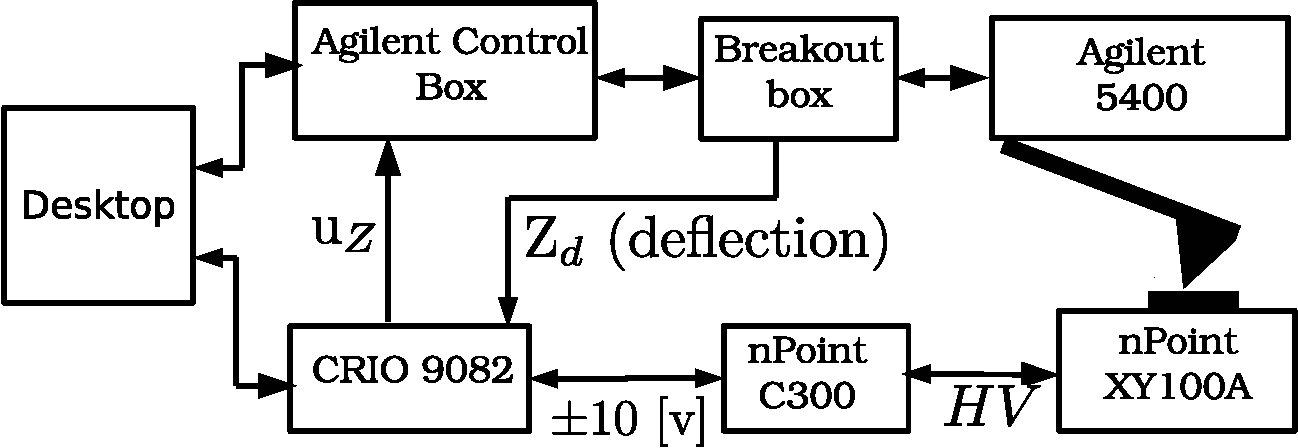
\includegraphics[width=1\columnwidth]{figures/exp_setup.pdf}
  \caption{Schematic diagram of the expermental AFM setup.}
  \label{fig:exp_setup}
\end{figure}

% =========================================================================
\section{Experimental setup} \label{sec:experimentalSetup}
% =========================================================================
Our experimental setup, illustrated in Fig.~\ref{fig:exp_setup},
consists of an Agilent 5400 AFM  retrofitted with an nPoint NPXY100A
piezoelectric stage, a cRIO-9082 embedded controller (National
Instruments), and a standard desktop computer. 


Through a breakout box, the Agilent 5400 provides access to the $z$-axis deflection signal. When the Agilent software is set to open-loop mode, a $\pm10$~volt input on the standard control box allows control of the $z$-axis of the N9524a piezo scanner, which has a total range of 7 $\mu$m.
Initial (course) engagement of the tip to the
sample is performed using the PicoView software before control is handed over to
the custom controllers.
	
All control logic is programmed using LabVIEW 2019 and compiled to a Xilinx
Spartan-6 LX150 Field Programmable Gate Array (FPGA) inside the cRIO-9082. The
cRIO includes a 16-Bit, 100 kHz NI-9215 analog-to-digital input module and a
16-Bit, 100 kHz NI-9263 digital-to-analog output module. All control loops are
implemented using a 25 kHz sampling rate.

% =========================================================================
\section{Control}\label{sec:control}
The control structure for each axis is different. For the $X$-axis, we use a
state space controller. It is described fully in \cite{braker_afmmpc_2019} and
achieves a bandwidth of about 150 Hz, which is over 1/3 of the first $X$-axis
resonance at 350 Hz.
\todo{Not sure how to give a deeper summary without getting to much into the weeds.}


The control law used for the $Y$-axis is a simple PI controller of the
form
\begin{equation}
  \frac{U(z)}{E_Y(z)}=D(z) = \frac{K_Iz}{z-1},
  \label{eqn:dzI}
\end{equation}
where, the error signal $E_Y(z) = Y(z)-R_Y$.

\todo{Should I implement something better for $Y$-axis, e.g., cancel complex
  pole-zeros at 350 hz and add notch filter???}

The $Z$-axis control is slightly more complicated than the simple $Y$-axis
integral controller and is described in the following subsection.
\subsection{Z-axis Control Design}\label{sec:zaxis_cs_control}
The main challenge to increasing the $Z$-axis bandwidth is the bending mode
resonance at 215 Hz, which can be seen in the FRF from $u_Z$ to $Z_{d}$ in
Fig.~\ref{fig:z_control} (blue curve). We address this by inverting the complex
pole-zero pair at 215 Hz. Thus, the entire $Z$-axis controller consists of a PI
controller, $D_I(z)$ cascaded with the resonance inversion, $D^{-1}(z)$, as shown in Fig.~\ref{fig:afm_bd_dinv}. The DC-gain
of $D$ is (approximately) the same as the DC-gain of the plant.
The inclusion of $D^{-1}$ allows us to substantially increase the PI gain and
achieve a closed-loop bandwidth of about 480 Hz. This is the black curve in Fig.~\ref{fig:z_control}.


There are multiple advantages to this method: first,
an inverse compensator still makes sense as a feedforward, open-loop compensator
if the feedback path is broken. This situation can and does occur during parts
of the CS cycle. Second, the inverse compensator
requires no tuning as it is defined only by a fit to the measured FRF.

One challenge to the inversion approach is both the system gain and resonance at 215~Hz
changes not only day-to-day but also (and especially) when changing cantilevers and our inversion is not robust to this. However, because $D^{-1}$ is defined purely by a second order fit to a small band of the FRF, updating the compensator can be automated.
\todo{What else to say here?}


\begin{figure}[t!]
  \centering
  \includesvg[width=1\columnwidth]{figures/z_control_design.svg}
  \caption{FRFs of the $Z$-axis. The blue curve is the open loop response from $u_Z$ to deflection. By inverting the bending mode at 215~Hz, we achieve the black curve in closed-loop.}
  \label{fig:z_control}
\end{figure}


\begin{figure*}
  \centering
  \includesvg[width=1\textwidth]{figures/MIMO_CL_uxuy.svg}
  \caption{MIMO closed and open loop FRFs, showing the dramatic affect on $G_{Z,u_X}$ and $G_{Z,u_Y}$ when the feedforward compensators are used for the $X$ and $Y$ axes.}
  \label{fig:mimo_frf_uxuy}
\end{figure*}

\begin{figure*}[t]
  \centering
  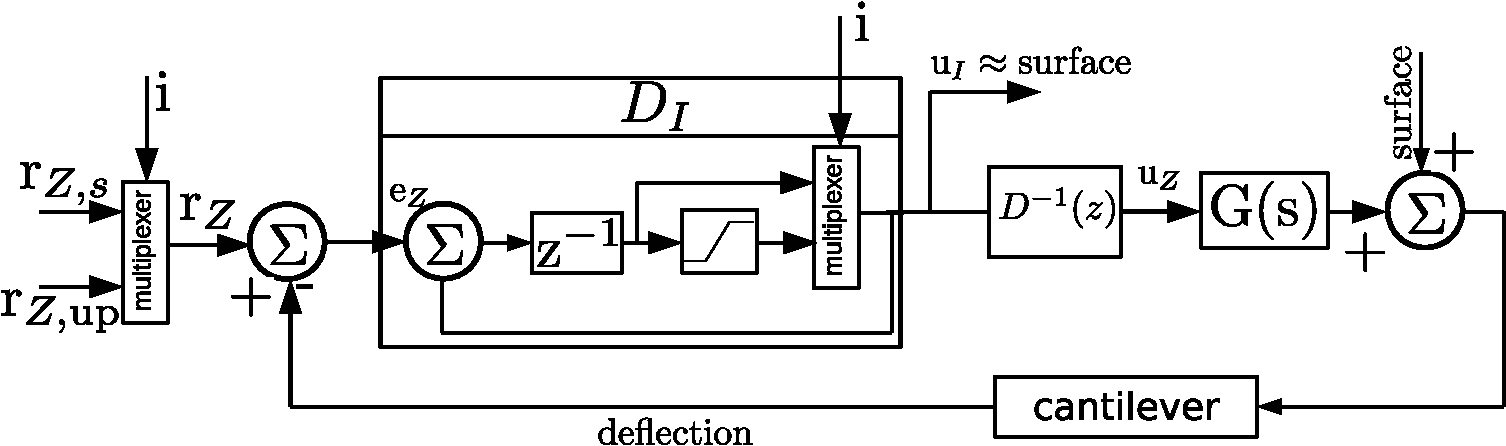
\includegraphics[width=0.75\textwidth]{figures/AFM_loop_z.pdf}
  \caption{Block diagram of the $Z$-axis control loop. The anti-windup is active
    for decision index $i\in\{0,1,5\}$, which correspond to states such that
    $r_Z=\rzup$.}
  \label{fig:afm_bd_dinv}
\end{figure*}

% One cause for such different gains is variation in the length of the cantilever
% (and possibly how the laser was adjusted). This is illustrated in
% Fig.~\ref{fig:z_axis_gain}. Here, we consider a cantilever with length $h$ that
% rests on the surface of some specimen with a nominal angle of $\theta$. In this
% drawing, the laser is perpendicular to the sample surface. Given a vertical
% perturbation $\Delta z$, we have that
% \begin{equation}
%   \Delta \alpha \approx \frac{d}{h} \Delta z,
% \end{equation}
% where $d$ is the distance from the cantilever to the detector and
% $\Delta \alpha$ is the change in position of the incident laser spot on the
% detector. Thus, given the same change in the vertical position, we will see a
% larger change in the deflection signal for a shorter cantilever. In other words,
% a short cantilever will exhibit a larger DC-gain in the $G_{u_Z,Z_d}$ transfer
% function.
% \begin{figure}
%   \begin{minipage}[t]{.46\textwidth}
%     % L B R T
%     \includesvg[width=1\textwidth]{figures/z_cant_evolution.svg}
%     \caption{FRFs of three different cantilevers, showing substantial
%       differences in the DC-gain and smaller, but still significant differences
%       the frequency of the modes.}
%     \label{fig:z_evolution}
%   \end{minipage}
%   \hfill
%   \begin{minipage}[t]{.46\textwidth}
%     % L B R T
%     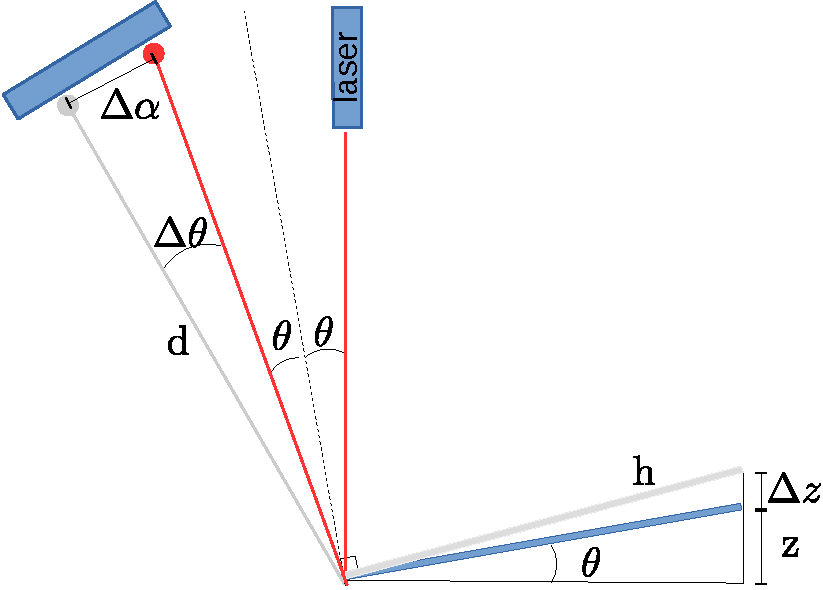
\includegraphics[width=1\textwidth]{figures/z_axis_gain_schematic-crop.pdf}
%     \caption{Schematic drawing of how the length of the cantilever affects the
%       $z$-axis gain.}
%     \label{fig:z_axis_gain}
%   \end{minipage}
% \end{figure}

% Fig.~\ref{fig:z_evolution} shows the frequency response of $G_{u_Z,Z_d}$ near
% the bending mode for three different cantilevers. Cantilevers (A) and (B) are
% both AppNano SICON cantilevers and have a nominal length of 450 microns.
% Cantilever (C) is an NCLR and has a nominal length of 225 microns.
% Interestingly, the SICON cantilevers show substantial variation. Unfortunately,
% the manufacture does not provide a tolerance on the nominal length, so it is
% difficult to tease out whether that variation is due to manufacturing
% variability or other factors not explained by this analysis.

% Notably, the frequency of the pole and zero do appear to shift and our inversion
% scheme is not robust to this. To deal with this, I have built a (mostly)
% automated system ID routine into the imaging software. This routine is a
% specialized version of the techniques described previously in
% Chapter~\ref{chap:modeling}. First, it obtains an FRF of the bending mode over a
% frequency range spanning 180~Hz to 240~Hz (the same set of points as in
% Fig.~\ref{fig:z_evolution}). The input and output sinusoids are demodulated in
% quasi-realtime as they come off the FPGA. Once this is complete, a 2-pole,
% 2-zero transfer function model of the form
% \begin{equation*}
%   \hat{D}(z) = k \frac{z^2 + b_1z + b_o}{z^2 + a_1z + a_o}
% \end{equation*}
% is fit to the FRF, using the same optimization scheme as \eqref{eqn:logfit}.
% This is done inside the LabView VI by calling a custom DLL, which leverages
% CMPFIT~\cite{cmpfit,markwardt_mpfit_2009}, a
% Levenberg-Marquardt~\cite{more_levenberg_1978} routine written in C. To promote
% a stable fit, the optimization enforces the necessary conditions that
% \begin{align*}
%   |a_1| &< 2, \quad  |a_o| < 1\\
%   |b_1| &< 2, \quad  |b_o| < 1.
% \end{align*}
% The routine then checks that both the poles and zeros are indeed stabile, saves
% the data to a JSON file and passes the transfer function parameters into the
% imaging portion of the application which finally uploads the parameters into the
% FPGA imaging bitfile. Optionally, one can by-pass this step and simply load the
% previously saved JSON file.

% One of the benefits of this approach is that the DC-gain of the transfer
% function $G_{u_Z,Z_d}$ becomes (approximately) normalized to unity, which makes
% re-tuning the control system after changing tips far easier to non-existent. The
% benefit to automating the process is that it drastically reduces the friction
% required to obtain an up-to-date compensator, which means that an up-to-date
% compensator is more likely to be used~\cite{abramovitch_25years_2015}.


% Fig.~\ref{fig:afm_bd_dinv} shows a block diagram if the $Z$-axis control loop.
% We point out a small change from Chapter~\ref{chap:cs_init}: the addition of
% $D^{-1}(z)$ changes the correct signal to use to represent the sample surface.
% If we take the output of the entire compensator, $u_Z=D_ID^{-1}e_z$, then we
% will get a lot of wiggles in the resulting signal. Rather, we need to take only
% the output of the integrator to represent the surface.
% % \begin{figure}
% %   \centering
% %   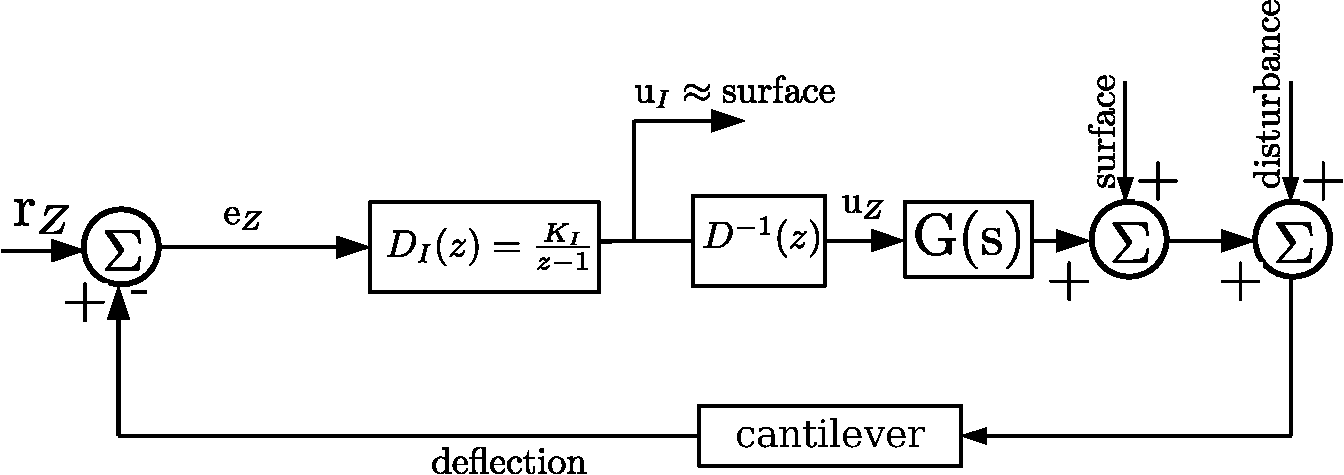
\includegraphics[width=1\columnwidth]{figures/AFM_loop_Dinv-crop.pdf}
% %   \caption{Block diagram of the $Z$-axis control loop with the inverse
% %   compensator. }
% %   \label{fig:afm_bd_dinv}
% % \end{figure}
% \begin{figure*}[t]
%   \centering
%   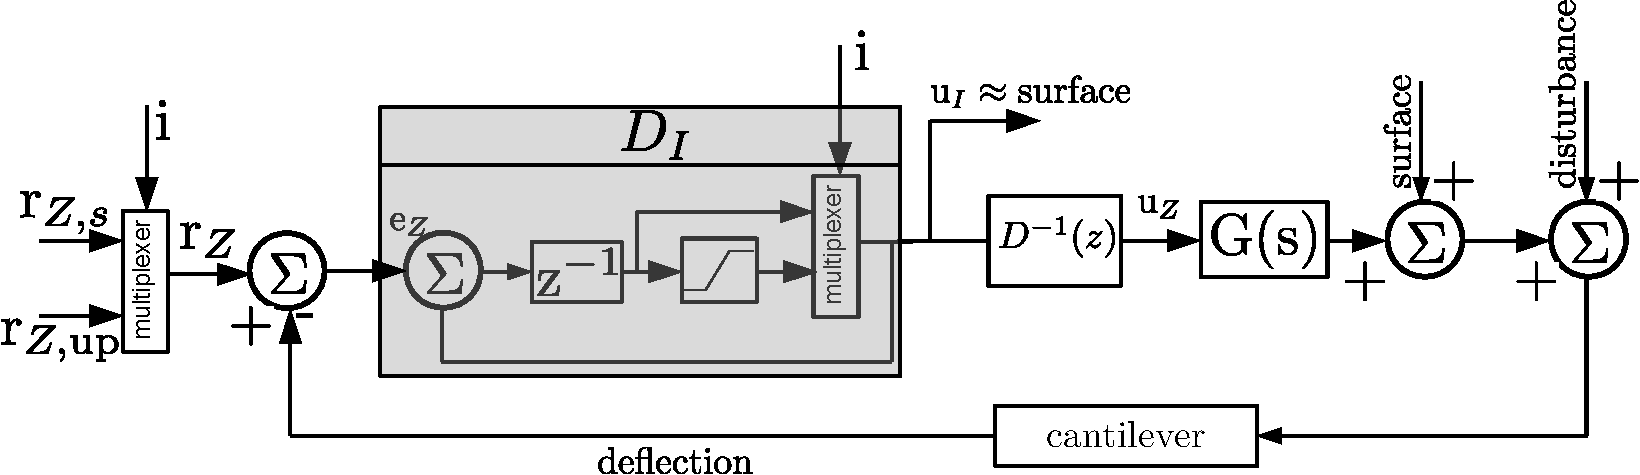
\includegraphics[width=0.75\textwidth]{figures/AFM_loop_Dinv_antiwup-crop.pdf}
%   \caption{Block diagram of the $Z$-axis control loop. The anti-windup is active
%     for decision index $i\in\{0,1,5\}$, which correspond to states such that
%     $r_Z=r_{Z,\textrm{up}}$.}
%   \label{fig:afm_bd_dinv_final}
% \end{figure*}


% It should be noted that this control is sufficient to eliminate the limit-cycle
% behavior described in Section~\ref{sec:aproachspeed}:

% % \begin{figure}[tbhp!]
% %   \centering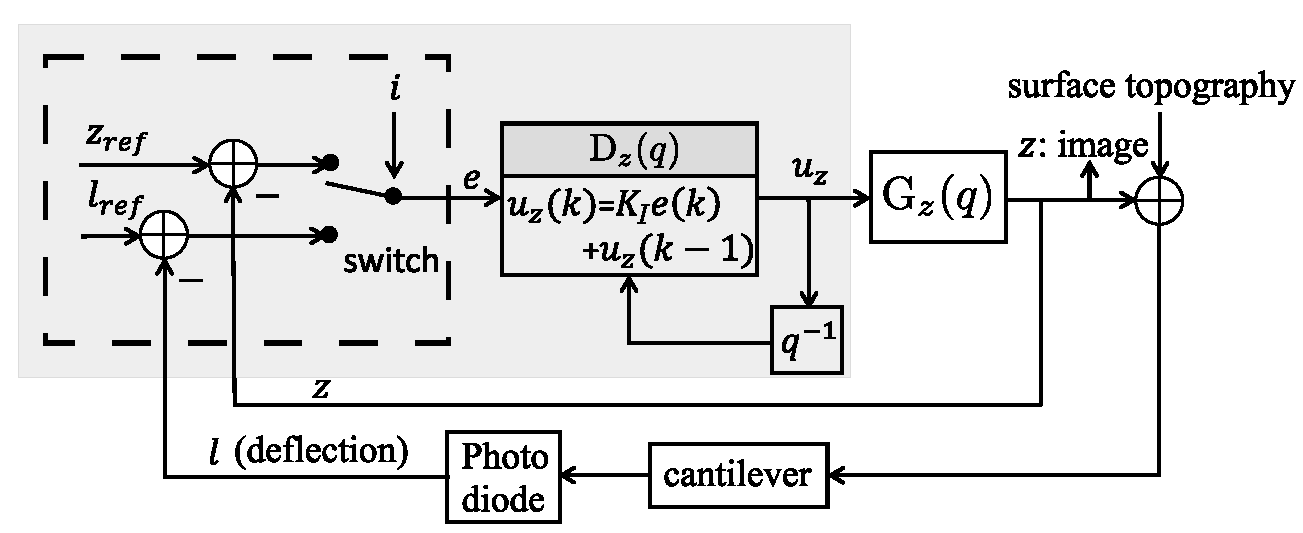
\includegraphics[width=3.0in]{figures-SBA/uz_multiplexer_KI_anderssonLab2}
% %   \caption{The $z$-piezo movement is driven by switching between feedback from
% %   the $z$-axis position signal and from the deflection signal. The shaded area
% %   represents the digital control system, while the non-shaded region is the
% %   physical system.}
% %   \label{fig:zMultiplex_anderssonLab}
% % \end{figure}
	
% As illustrated in Fig.~\ref{fig:zMultiplex_anderssonLab}, the voltage applied to
% the $z$-piezo is adjusted by switching the feedback signal between the $z$-axis
% position sensor (when the tip is off the surface) and the deflection signal
% (when the tip is engaged). The difference equation associated with
% \eqref{eqn:dzI} for the $z$-axis is
% \begin{equation}
%   u_z(k) = K_Ie(k) + u_z(k-1).
%   \label{eqn:intdiff}
% \end{equation}

% In the $z$-axis position control mode, the $z$-axis position is controlled to a
% fixed value $z_{ref}$ which, in general, is slightly above the sample surface.
% The difference between the measured $z$-axis position and $z_{ref}$,
% ${e(k) = z_{ref} - z(k)}$, is used as the error signal. In the deflection
% control mode, when the tip is in contact with the sample, the deflection signal
% is controlled to a fixed value $l_{ref}$ to ensure a constant tip-sample force.
% The sample surface acts as a disturbance to the control loop. Therefore, the
% $z$-axis position measurements can be taken to represent the surface topography
% of the sample. In this case, the difference between the measured deflection and
% $l_{ref}$ is the error, $e(k) = l_{ref} - l(k)$.
	
% We note that the $z$-axis control described here operates the AFM in constant
% force mode during imaging. It is straightforward to perform scanning under
% different AFM modes, such as tapping mode, simply by adjusting the signals and
% control involved in the vertical loop.

\subsection{Feedforward Control}\label{sec:ff_control}
In our AFM, there is a strong coupling between the horizontal axes and vertical deflection. Fig.~\ref{fig:mimo_frf_uxuy} shows a MIMO FRF for $u_X$ and $u_Y$ to the outputs in each axis. The dotted black curves are the open loop responses and the dashed red curves are the nominal closed-loop responses. Though the $Z$-direction inputs are not shown, the closed loop responses include the $Z$-axis controller. Note that, especially for $H_{z,u_X}$, the closed-loop response is barely improved over the open loop response and in particular, there is a sharp resonance at 215~Hz and 505~Hz. To deal with this, we employ two different strategies for CS and raster scanning.

For CS scanning, we insert a feed-forward filter with two notches, one at 215~Hz and the other at 505~Hz. We design a similar feed-forward filter for the $Y$-axis. Both filters are shown in Fig.~\ref{fig:mimo_frf_uxuy} as the solid pink curves and the resulting overall FRF is shown as the solid blue curves. Particularly for $H_{z,u_X}$, these filters result in a dramatic reduction in the cross coupling. A similar affect could be achieve by using a simple low-pass filter. However, to achieve the same 40~dB of attenuation of the mode at 215 Hz, would require, e.g., that a two-pole LPF have its cut-off frequency at about 20~Hz. 

For raster scanning, we use a truncated Fourier series, where each Fourier coefficient is scaled by the inverse of the closed-loop FRF at the corresponding frequency. We truncate this series such that the highest frequency is smaller than 200 Hz. See, e.g., \cite{clayton_review_2009} for more details on this strategy. Note that these scheme implies that the effective bandwidth of the $X$-axis controller is higher while raster scanning than while CS-scanning. On the other hand, it also implies that the for faster scan rates, fewer Fourier coefficients are used, and so the approximation to a triangle wave is worse.

% =========================================================================
\section{Implementation}\label{sec:implementation}
% =========================================================================
	
% =========================================================================
\subsection{State machine}
Implementing the $\mu$-path scheme involves operating the AFM in several
distinct stages. In the $xy$-direction, the system must transition from tracking
a step command (in the transition to a new measurement location) to tracking a
scan pattern. For our simple integral controller, this only involves changing
the reference signals $x_{ref}$ and $y_{ref}$.
In the $z$-direction, the system
must transition between tip descent, surface scanning, tip retraction, and
maintaining a $z$-axis position.

	
Transition between, and operation in, these different stages is implemented as a
simple state machine, summarized in Table~\ref{tab:cs_tasks}. 
In the following, $r_X$ and $r_Y$ refer to the references for the $X$ and $Y$ axes while $r_{Z,s}$ and $\rzup$ refer to the $Z$-axis setpoints during scanning and retraction, respectively.

\begin{table}
  \centering
  \caption{Summary of the tasks for $\mu$-path scanning.}
  \begin{tabular}{lccc}
    state & $X$,$Y$ & $Z$ & next-state\\
    \toprule
    (1) $XY$-move & setpoint & $r_Z = \rzup$ & (2)\\
    (2) tip-engage & setpoint & $r_Z = \rzs$ & (3)\\
    (3) pre-scan & ramp & $r_Z = \rzs$ & (4)\\
    (4) $\mu$-path scan & ramp & $r_Z = \rzs$ & (5)\\
    (5) tip up & setpoint & $r_Z = \rzup$ & (1)\\
  \end{tabular}
  \label{tab:cs_tasks}
\end{table}
Two cycles of this sequential process are illustrated by the time series in
Fig.~\ref{fig:mupathsignaltrajectory}. The following subsections describe in
more detail several features of the CS scanning process.
  
\begin{figure}[t!]
  \centering
  \includesvg[width=1\columnwidth]{figures/cs_cycle.svg}
  \caption{Several CS cycles. Each state is indicated by color.}
  \label{fig:mupathsignaltrajectory}
\end{figure}

\subsection{Cantilever does not need to fully disengage.}
\todo{Not clear to me yet that friction is useful if I scan parallel to cantilever.
  Also not clear to me that the normal force and shear force are orthogonal concepts.
  Maybe the macroscopic analogy breaks down, but thinking of a knife pushed into a surface and then dragged...}
In our initial implementation \cite{braker_hardware_2018}, we insisted that the during tip-retraction
(state-5), the cantilever tip should fully break contact with the surface. Here,
we impose no such requirement. Rather, we change the $Z$-setpoint during
tip-retraction to only pull away far enough that the deflection signal stays low
(i.e., below the scanning setpoint), even while we run across the surface.
We choose \rzup so that the interaction between the tip and sample becomes purely adhesive.
In general, stable imaging in is not possible at \rzup and complete dis-engagement occasionally occurs.


The change in setpoints is achieved via the multiplexer in Fig.~\ref{fig:afm_bd_dinv}
which selects either the scanning setpoint $r_{Z,s}$ or the retraction setpoint
$r_{Z,\textrm{up}}$ based the current state.
When dis-engagement does occur, the $Z$-axis control loop implements an anti-windup scheme.



% Ultimately the concern is damage to the sample and tip,
% which is caused by the force imparted by the cantilever probe
% \cite{clayton_review_2009}. The deflection signal, though un-calibrated (meaning
% it does not directly lead to a value in $kN$), is proportional to that force,
% because it is proportional to how much the cantilever is bent. I.e., a large
% (towards $+\infty$) deflection implies the spring force of the cantilever is
% pushing hard into the sample, thereby inducing damage. In a typical imaging
% scenario, we choose a deflection setpoint, (say $0.15$~[v], as in
% Fig.~\ref{fig:z_drift}), and have in some way decided that this is sufficient,
% all else being equal, to not damage things too much.


\subsection{The pre-scan}
\begin{figure*}
  \begin{subfigure}{.33\textwidth}
    \includesvg[width=1\textwidth]{figures/zbounce_uz_example.svg}
    \caption{ }
    % \label{fig: }
  \end{subfigure}
  \begin{subfigure}{.33\textwidth}
    \includesvg[width=1\textwidth]{figures/prescan_uz_example.svg}
    \caption{ }
    \label{fig:uz_prescan}
  \end{subfigure}
  \begin{subfigure}{.33\textwidth}
    \includesvg[width=1\textwidth]{figures/prescan_zbounce_PSD.svg}
    \caption{ }
    % \label{fig: }
  \end{subfigure}
  \caption{(a) A ``$Z$-bounce'' experiment where the $XY$-stage is motionless
    and the cantilever is repeatedly engaged and disengaged. (b) One cycle of a
    tightly packed set of CS-cycles where the movement between each measurement
    location is 0. (c) PSDs from the portions of the trajectories which are
    colored blue and turquoise, averaged over many such cycles, demonstrating
    that the scan process itself reduces vibration in the $Z$-axis.}
  \label{fig:prescan_difference}
\end{figure*}
After the tip-descent, we begin scanning in a ``pre-scan'' phase (state (3)).
During this phase, 

To motivate, this consider Fig.~\ref{fig:prescan_difference}. The left panel
represents what we call a ``$Z$''-bounce experiment, where the $XY$-stage stays
motionless, but we repeatedly retract and re-engage the tip with specimen,
exactly as we would in a CS scan. The right panel represents a single cycle from
specialized CS pattern, where the $\mu$-paths are still 500 nm long, but the
paths are separated by 0 pixels.
In this case, the specimen is freshly cleaved
mica.
The goal here is to eliminate (i) any oscillations which arise from the
$XY$-move and (ii) to have a perfectly flat surface to scan over so that
there are as few disturbances as possible entering the control loop. Finally,
the left panel of Fig.~\ref{fig:prescan_difference} shows the PSDs of the left
and right panels (but averaged over many similar cycles). Note that the PSD is
only computed from the combination of the blue and turquoise signals.

What we see then, is that, for some unknown (to me) reason, scanning reduces the
amount of energy that shows up near 215 Hz. The idea behind the pre-scan is to
take advantage of this. The pre-scan phase is relatively long (150 samples),
especially for the faster scan rates. However, the pre-scan also allows us to
eliminate the over-scan at the end of the $\mu$-path, because by the time we are
ready to start taking data, the $X$-axis is already in quasi-steady-state. For
the current control design, the required over-scan is about 90 samples (which
can be computed from the steady-state error of the closed-loop system to a
ramp), which means the pre-scan incurs an effective overhead of about 60 samples
per $\mu$-path.

% The tip settling (pre-scan) period could likely be much shorter if we a had a
% $Z$-axis position sensor. Part of the reason it is so long is that, despite not
% pulling the cantilever completely away from the sample, there is still a small
% drift transient, as can be seen Fig.~\ref{fig:uz_prescan}. We would like to at
% least give the major part of that drift transient time to die out. With a
% position sensor, we would not care about the drift transient: the control signal
% drifts to keep the $Z$-position constant.

% \section{Post-processing}\label{sec:post_process}
% Here, we discuss how we post-process the raster and CS images.

% \subsection{Aligning images via cross-correlation}\label{sec:align}
% To get metrics that are meaningful in any sense, we need the master image and
% the comparee to be aligned. We take two steps to help ensure this. First, during
% each batch of images, the nPoint stage remains under closed loop control.
% Between images, the FPGA control loop idles in state-0, as discussed above in
% Section~\ref{sec:idle_0}. This was not necessary duing the initial
% implementation because then, the nPoint stage was controlled by the nPoint PI
% controller. While this helps things substantially, there is still an alignment
% issue between subsequent images, which I believe stems from the original Agilent
% piezo tube, which is a three axis tube. The $XY$-axes of the tube are
% uncontrolled during imaging, and in fact, after a firmware ``upgrade'', the
% option to close the $XY$-loop has been grayed out in the PicoView software.

% To help deal with this, we compare sub-slices of the master image and the
% comparee. The results in this chapter use a sub-image obtained by removing a
% border of 25 pixels from each edge. Thus, for the purposes of comparison, the
% original 512$\times$512 pixel image becomes a 462$\times$462 pixel image. Let
% $X$ represent the original, master image and ${\tilde X=X_{25:-25, 25:-25}}$,
% using Python notation. To find the correct subslice of the comparee, we use a
% two dimensional cross-correlation, which is defined as
% \begin{equation}
%   Z_{k,\ell} = \sum_{m=0}^{M-1}\sum_{n=0}^{N-1} \tilde{X}_{m-k, n-\ell}Y_{m-k, n-\ell}.
% \end{equation}
% where $Y$ is the comparee.

% The index of the maximum value of the matrix $Z$
% \begin{equation}
%   (i^*,j^*) = \textrm{arg~} \max_{i,j}Z_{i,j}
% \end{equation}
% corresponds to the lower left corner of the correct subslice. Thus, the
% comparisons will computed against $\tilde{Y} = Y_{i^*:i^*+487, j^*:j^*+487}$.
% For an example of this in action, see the Fig.~\ref{fig:baseline_errors} in the
% next section.

% Unfortunately, the mis-alignment is not simply constant offset, but rather
% drifts over time. This can be seen, e.g., in Fig.~\ref{fig:rast_aligned_0p5}.
% Thus, while the technique described here mitigates the issue, it does not fully
% eliminate the problem.


\section{Metrics}\label{sec:rdi}
In section~\ref{sec:results} we use three metrics to asses our results.
The first two seek to quantify image quality of two images. 
Define a master image as $X$ and a reconstruction or corrupted version as $Y$, with each having $s\times h=m$ pixels.
Let $x=\textrm{vec}(X)$ and $y=\textrm{vec}(Y)$. Let $L$ be the dynamic range of the master image $x$.
Then the peak signal to noise ratio (PSNR) is given by
\begin{equation*}
  \text{PSNR}(x,y) = 10\log_{10}\frac{L^2}
  {\sqrt{\frac{1}{p^2} \sum_{i=1}^{m}( x_{i} - y_{i})^2 }}.
\end{equation*}

The goal of the SSIM is to compare two image's structure, luminescence, and contrast and is built up from the means ($\mu_x$ and $\mu_y$), standard deviations ($\sigma_x$ and $\sigma_y$), and covariance ($\sigma_{xy}$) of the image vectors $x$ and $y$.  
The variation of the SSIM used in this paper is defined as
\begin{equation*}
  \text{SSIM}(x,y) = \frac{(2\mu_x\mu_y + C_1)(2\sigma_{xy}+C_2)}
  {(\mu_x^2 + \mu_y^2 + C_1)(\sigma_x^2 + \sigma_y^2 + C_2)}
\end{equation*}
where the constants $C_1$ and $C_2$ are regularizing constants to prevent singularity if, e.g., $\mu_x=\mu_y=0$.
We use the default values suggested in \cite{wang_image_2004} of $C_1=(0.01L)^2$ and ${C_2=(0.03L)^2}$, where again, $L$ is the dynamic range.
In general two images which are identical will yield an infinite PSNR and an SSIM of 1.

\subsection{Limitations of SSIM and PSNR}\label{sec:limits}
What kind of numbers are reasonable to expect from the SSIM and PSNR metrics?
To answer this question, we compare a sequence of 1~Hz raster scans.
In this experiment, (Fig. \ref{fig:rast_unaligned_1}) we took 6 raster scans of the same 5 by 5 micron
square of the CS-20NG sample grating. These scans were taken sequentially and
the NPXY100A remained in closed-loop throughout the process.
Fig.~\ref{fig:rast_unaligned_1} shows the error between the master
image and the remaining 6 images.
Temporally, the images are order left-to-right and top-to-bottom.
Thus we can see, both visually and via the metrics, that in Fig.~\ref{fig:rast_unaligned_1} the mis-alignment
grows over time. 
\todo{Should probably remove this entire section?}

Taking the first scan as the master, we compute the PSNR and SSIM
metrics. The best PSNR here is 16.57 and the worst is 9.02.
The best SSIM is 0.54 and the worst is 0.28.

\begin{figure}[t!]
  % ------------ 1.0 Hz ---------------------
  \begin{subfigure}{.48\textwidth}
    \includesvg[width=1\textwidth]{figures/baseline_errors_noalign_1Hz.svg}
    \caption{1.0~Hz, no alignment.}
    \label{fig:rast_unaligned_1}
  \end{subfigure}
  \hfill
  \begin{subfigure}{.48\textwidth}
    \includesvg[width=1\textwidth]{figures/baseline_errors_aligned_1Hz.svg}
    \caption{1.0~Hz, with alignment.}
    \label{fig:rast_aligned_1}
  \end{subfigure}
% 
  \caption{Errors between a ''master'' and 6 different raster scans, all taken
    sequentially and at a scan rate of 0.5 Hz. (a) Errors without alignment (b)
    The same data as above in (a) but aligned via cross correlation.}
  \label{fig:baseline_errors}
\end{figure}

Next, using a cross-correlation alignment technique
% discussed in Section~\ref{sec:align},
we aligned the master image with a sub-slice of each of
the remaining 6 (the sub-slice removes 25 pixels from each side). Again, we
computed the PSNR and SSIM. These results are shown in
Fig.~\ref{fig:rast_aligned_1}, which again shows the errors between the
aligned master and the remaining 6 images. Although the situation is improved
compared to the un-aligned images, there is still noticeable stretching,
particularly in the $Y$-direction. Notably, with the alignment technique,
the SSIM lies between 0.7 and 0.73 and the PSNR ranges from 22.51 to 24.99 and appears more stable in time.




% Due to this unfortunate drift, in Section~\ref{sec:results:final}, we will use a
% 1~Hz scan as the baseline image. Hopefully, this will give a decent trade-off
% between having an image with minimal drift and scanning slowly enough that it
% accurately represents the sample grating. Due to the improved $Z$-axis
% bandwidth, a 1~Hz scan should still have better (or at least comparable) quality
% than the 0.25~Hz scan taken in Chapter~\ref{chap:cs_init}. Additionally,
% Fig.\ref{fig:rast_aligned_1} provides us with an (approximate) upper bound for
% our expectations when looking at the experimental results in
% Section~\ref{sec:results:final}.

\subsection{A new metric}
\begin{figure}[t!]
  \centering
  \includesvg[width=1\columnwidth]{figures/damage_illustration.svg}
  \caption{The RDI metric defined in \eqref{eqn:RDI} penalizes everything in the
    red shaded region and does not penalize anything in the un-shaded region.}
  \label{fig:damage_illustrate}
\end{figure}

Th PSNR and SSIM metrics only assess the similarity of two images.
However, in AFM imaging, pure image quality is not the
only concern, particularly for delicate samples. What is needed is a figure of
merit for how much damage was done to specimen during the imaging process. While
this is not really a concern while imaging a hard calibration grating, it plays
a prominent role biological samples~\cite{ando_highspeed_2008}. In general,
damage occurs while scanning into an uphill region, which results in a positive
deflection signal. The actual damage done by a given $Z_d$ will depend on the
spring constant of the cantilever and the softness of the specimen. Nonetheless,
we can use the positive deviations of $Z_d$ as a relative measure of damage
between different scan speeds or scanning methods, for a given cantilever and
specimen. This motivates a metric we term the relative damage index (RDI), which
we define as
\begin{align}
  \text{RDI} &= \frac{1}{T_s}\sum_{k\in I} \frac{1}{k} \left(Z_{d,k} - r_{Z,s}\right)^2 \label{eqn:RDI}\\
  I &= \{k: k\in[0,~N-1],~ Z_{d,k}-r_{Z,s} > 0 \} \nonumber
\end{align}
where $N$ is the total number of samples in a given scan, $Z_{d,k}$ is the
deflection signal at sample $k$ and $r_{Z,\textrm{s}}$ is the scanning setpoint.
The RDI is basically the power in positive deflection. By excluding negative
values of the deflection, we do not penalize the CS algorithm while it is
re-engaging with the specimen \emph{unless} it overshoots the scanning setpoint,
which we do want to penalize. This is illustrated in
Fig.~\ref{fig:damage_illustrate}, which shows several CS cycles with a poorly
tuned controller. Only deflection signals in the red-shaded region will be
penalized by the RDI.

\section{Experimental Results}\label{sec:results}
We took scans of the CS-20NG sample grating over an area with holes on a 500 nm
pitch. The holes are 20 nm deep.
We scanned 5 micron by 5 micron images with 512
lines each, yielding 512 by 512 pixel images. As before, the $\mu$-path scans
are 500 nm long, as this allows us to work around the lack of a $Z$-axis sensor.
This yields a $\mu$-path size of 52 pixels.

The free value of the deflections signal was approximately -0.6 volts and we set
the scanning reference to ${\rzs=-0.3}$~volts and the withdraw reference to
${\rzup=-0.8}$ volts. We set the $XY$-settle boundary to $\pm 0.05$
microns and required 20 samples within this boundary before moving to the
$Z$-engage state. The pre-scan length was 150 time steps.

\todo{Should I scan even faster??}

For the raster scans, we took scans at 1.0~Hz, 4.0~Hz, 5.0~Hz, 8.0~Hz and
10~Hz.  The CS scans we taken with scan velocities equivalent to raster scans of 1.0~Hz,
2.0~Hz, 4.0~Hz, 5.0~Hz and 8.0~Hz with sampling densities of 10~\% and 15~\%.
The cantilever was an AppNano SICON, with a
length of 450 microns and spring constant $k\in[0.02,~0.8]$~N/m.

The CS scans were reconstructed with BPVV. We set
$\sigma = 0.1$, $\mu_f=$TKT, $\alpha_v=$TKT and $\alpha_h=$TKTKT. The data remained scaled in terms of volts.

For the raster scans, we discard data from the re-trace and divided the
remaining data into 512$\times$512 bins based on the \xc and \yc sensor
measurements. We then average the data in each bin to obtain the value of one
pixel. To remove the affects of piezo creep and sample tilt, we then de-trend
each individual line. De-trending each line causes the flat portion between the holes in the horizontal direction to appear at a different height than the flat portion between holes in the vertical direction. 
To remove this effect, we select a column of
pixels on the left and right side of each image that does not cross any holes
(i.e., a vertical line through the flat area), register each scan line to a
common height along these columns. This step eases comparison with the CS scans
and was inspired by a feature in \texttt{SPIW} \cite{spiw}.

As a final step, we subtract the mean from each CS and raster image, so that
they can all be mapped to the same color intensity in the images. The color maps
represent a range of $\pm$20 nm.


The resulting images are shown in Fig.~\ref{fig:resultsF1_images}. The rows of
pixels indicated by the red lines are shown Fig.~\ref{fig:pixel_rows}.

% The sub-slice removed a 30 pixel
% boundary from each edge. Despite this alignment, the middle pixels tend to show
% a smaller error than those towards the top and bottom, which is similar to the
% affect observed before in Fig.~\ref{fig:baseline_errors}.

For each raster scan and each CS scan, we computed the SSIM, PSNR (both with
default parameters) using the 1~Hz scan as the master and also computed the RDI
metric. These are collected in table ~\ref{tab:rast_vs_cs_v1}.

\begin{figure*}
  \includesvg[width=1\textwidth]{figures/cs_raster_images_4-26-2019}
  \caption{Raster and compressed sensing images of a 5 micron square area of the
    CS-20NG grating. All images are 512$\times$512 pixels. The rows of pixels
    indicated by the red line are shown in Fig.~\ref{fig:pixel_rows}.}
  \label{fig:resultsF1_images}
\end{figure*}



\begin{table}[t!]
  \centering
  \caption{Performance metrics for raster and CS scans.}
  \begin{tabular}{cccccc}
    type &  rate (Hz) & PSNR & SSIM & time [s] & damage\\
\toprule
raster & 1.00 & Inf & 1.00 & 512.0 & 1.06\\
raster & 4.00 & 21.96 & 0.72 & 128.0 & 8.11\\
raster & 5.00 & 22.07 & 0.72 & 102.4 & 10.86\\
raster & 8.00 & 22.52 & 0.71 & 64.0 & 18.58\\
raster & 10.00 & 21.23 & 0.65 & 51.2 & 23.70\\
CS (10.02~\%) & 1.00 & 20.50 & 0.69 & 34.8 & 1.21\\
CS (10.02~\%) & 2.00 & 20.89 & 0.70 & 22.0 & 2.77\\
CS (10.02~\%) & 4.00 & 20.43 & 0.68 & 15.6 & 6.57\\
CS (10.02~\%) & 5.00 & 20.90 & 0.69 & 14.3 & 8.21\\
CS (10.02~\%) & 8.00 & 20.58 & 0.67 & 12.5 & 13.13\\
CS (15.02~\%) & 1.00 & 21.24 & 0.73 & 52.1 & 1.15\\
CS (15.02~\%) & 2.00 & 21.50 & 0.73 & 32.9 & 2.67\\
CS (15.02~\%) & 4.00 & 21.42 & 0.72 & 23.3 & 6.62\\
CS (15.02~\%) & 5.00 & 21.22 & 0.72 & 21.4 & 8.11\\
CS (15.02~\%) & 8.00 & 20.92 & 0.70 & 18.6 & 12.93\\

  \end{tabular}
  \label{tab:rast_vs_cs_v1}
\end{table}

\begin{table}[t!]
  \centering
  \caption{Breakdown of state times for the CS scans listed in
    Table~\ref{tab:rast_vs_cs_v1}. All times are in seconds.}
  \label{tab:final_state_times}
  \begin{tabular}{ccccccc}
    description & move & engage & pre-scan & scan & tip-up & total\\
\toprule
1.0 Hz, 10.02~\% &3.92 & 0.71 & 3.06 & 25.85 & 0.48 & 34.02\\
2.0 Hz, 10.02~\% &3.93 & 0.71 & 3.06 & 13.08 & 0.48 & 21.26\\
4.0 Hz, 10.02~\% &3.95 & 0.71 & 3.06 & 6.70 & 0.49 & 14.90\\
5.0 Hz, 10.02~\% &3.94 & 0.71 & 3.06 & 5.41 & 0.49 & 13.60\\
8.0 Hz, 10.02~\% &3.91 & 0.71 & 3.06 & 3.50 & 0.49 & 11.67\\
1.0 Hz, 15.02~\% &5.83 & 1.07 & 4.58 & 38.76 & 0.72 & 50.96\\
2.0 Hz, 15.02~\% &5.79 & 1.06 & 4.58 & 19.60 & 0.72 & 31.77\\
4.0 Hz, 15.02~\% &5.77 & 1.07 & 4.58 & 10.04 & 0.73 & 22.20\\
5.0 Hz, 15.02~\% &5.75 & 1.07 & 4.58 & 8.11 & 0.74 & 20.25\\
8.0 Hz, 15.02~\% &5.75 & 1.07 & 4.58 & 5.25 & 0.74 & 17.39\\

  \end{tabular}
\end{table}

\begin{figure*}[t!]
  \includesvg[width=1\textwidth]{figures/cs_raster_pixel_rows_4-26-2019.svg}
  \caption{Rows of pixels, as indicated by the red lines in
    Fig.~\ref{fig:resultsF1_images}. For clarity, not all images are included.}
  \label{fig:pixel_rows}
\end{figure*}

Unfortunately, the SSIM and PSNR metrics are not particularly illuminating. It
is easiest to see this by plotting PSNR and SSIM against total acquisition time,
which is shown in Fig.~\ref{fig:time_ssim} and ~\ref{fig:time_psnr}. There are several
inconsistencies. First, the 4~Hz raster scan has the lowest PSNR of all the
raster scans, while the 8~Hz scan has the highest. Second, all of the 15\% CS
scans except the 8~Hz version have as good or better SSIM numbers than the
raster scans. It makes no sense for a CS scan at a 5~Hz rate to have better
quality than a raster scan at a 5~Hz rate.

% It is interesting to also compare
% these numbers to the batch of 1~Hz raster scans we compared in
% Section~\ref{sec:limits}.
% The blue shaded bands of
% Figs~\ref{fig:time_ssim_psnr} indicate the mean of the SSIM and PSNR metrics
% from Section \ref{sec:psnr_ssim_limits} plus or minus one standard deviation.
% This seems to be further evidence that, at least for our experimental setup,
% these numbers are not especially meaningful.

\begin{figure*}[h!]
  \begin{subfigure}{0.33\textwidth}
    \includesvg[width=\textwidth]{figures/cs_rast_time_vs_ssim.svg}
    \caption{}
    \label{fig:time_ssim}
  \end{subfigure}
  \begin{subfigure}{0.33\textwidth}
    \includesvg[width=1\textwidth]{figures/cs_rast_time_vs_psnr.svg}
    \caption{}
    \label{fig:time_psnr}
  \end{subfigure}
  \begin{subfigure}{0.33\textwidth}
    \includesvg[width=\textwidth]{figures/cs_rast_damage.svg}
    \caption{}
    \label{fig:time_damage}
  \end{subfigure}
\caption{Metrics for raster scan and $\mu$-path scans at 10\% and 15\% sampling. (a) SSIM as a function of total acquisition time. (b) PSNR  as a function of total acquisition time. (c) RDI as a function of total acquisition time.}
    
  % \label{fig:time_vs_metrics}
\end{figure*}

Where CS seems to really shine is if we look at the RDI for a given time or scan
rate. This is plotted in Fig.~\ref{fig:time_damage}. For example, the 10~Hz
raster scan, which takes about 51 seconds, gives an RDI of 23.7. All of the CS
scans, except for the 15\% scan at 1~Hz (which is only 0.9 seconds longer) are
faster than the 10~Hz raster scan, yet have much lower RDI values, ranging from
1.21 to 13.13. Unsurprisingly, the relationship between scan speed and RDI is
quite linear. For the raster scans, the left panel of Fig.~\ref{fig:time_damage}
just plots the inverse relationship of the right panel, since scan time is
inversely proportional to raster frequency. This is not quite the case for the
CS scans due to the sub-sampling and the fixed overhead which does not scale
with scan rate (e.g., the amount of time for the $XY$-move etc remains
essentially constant for a given scan density).

What is surprising is that for the same scan rate, the CS scans have a lower RDI
than a raster scan at the same rate. One possibility is that the probability
that a given $\mu$-path will start on the flat portion of the grating, scan
\textit{into} a hole and then the tip withdraws before exiting the hole is
higher than the probability that a scan starts in a hole and exits the hole.
This would result in a lower RDI, because scanning \textit{out} of hole is what
the RDI penalizes.

From the left panel of Fig.~\ref{fig:time_damage}, we see that for a fixed RDI,
CS has a faster imaging acquisition rate. The amount of improvement is best if
we need a very low RDI: for example, if we want to hold the RDI below 2, then we
have to take the 1~Hz raster scan (512 seconds) while we can achieve the same
RDI via CS in about 52 seconds with the 15\% sampling, which is a speed
improvement of nearly 10. The higher of an RDI we are willing to tolerate, the
advantage of CS over raster narrows. For example, the 4~Hz raster scan and 5~Hz,
15\% CS scan have comparable RDI, but now CS is only about 6 times faster. This
is a result of the constant overhead imposed by the engage/disengage and
$XY$-move states in CS.

\subsection{Comparison to sub-line sampling}
Compressed sensing so far does not look good if we compare to subline sampling. The left panel of Fig.~\ref{fig:subline} shows a 5~Hz raster scan taken with 128 lines which takes approximately 25 seconds. We use that data to produce a 128 by 512 pixel image, and then use basic linear interpolation to fill produce a 512 by 512 pixel image. The CS image with the nearest acquisition time (15\% at 4~Hz) is shown in the right panel. The raster scan looks better and has basically the same RDI, and better SSIM and PSNR numbers. We conclude there is no reason to use CS.
\begin{figure}
  \includesvg[width=1\columnwidth]{figures/subline_vs_cs.svg}
  \caption{(left) A 128 line raster scan interpolated onto 512 lines. (left) the CS scan with the nearest time.}
  \label{fig:subline}
\end{figure}

\section{Conclusions}\label{sec:conclusions}
The main conclusion of this chapter is that with CS, it seems that we can
acquire images faster yet (putatively) with less specimen damage than is
possible with raster scanning, which we showed by introducing a new metric, the
RDI. Of course, a natural criticism is that we did not validate the RDI against
delicate specimens. We leave this as an area for future work.






%%%%%%%%% then the Bibliography, if any %%%%%%%%%
% \bibliographystyle{plain} % or "siam", or "alpha", etc.
\bibliographystyle{IEEEtran} % or "siam", or "alpha", etc.
% \nocite{*} % list all refs in database, cited or not
\bibliography{braker_bibs,Andersson_bibs,Yufans_bibs} % Bib database in "refs.bib"


%%%%%%%%% then the Appendices, if any %%%%%%%%%
\end{document}

